%%%%%%%
\subsection{Static scheduling}\label{s:Evaluation:HyperflowScheduler}

% \todo{Evaluation without task clustering}

The first prepared scenario is workflow execution without task clustering.
Its results allow to analyze the effectiveness and applicability of traditional scheduling algorithms for containerized environments.
In this scenario, two scientific workflows are considered:

\begin{itemize}[topsep=0pt]
  \item{
SoyKB (52 time consuming tasks),
}
  \item{
Montage2-v0.25 (619 smaller tasks).
}
\end{itemize}
Both have been chosen for their relatively small size in terms of task number and short enough completion times for repetitive runs.


The example execution traces of SoyKB workflow are shown in \cref{fig:evaluation:sched:soykb} and the numerical values of calculated metrics are presented in \cref{tab:metrics-sched-soykb}.


%%%%%%%
% SoyKB traces
%%%%%%%
% \begin{figure}[H]
% \centering
% 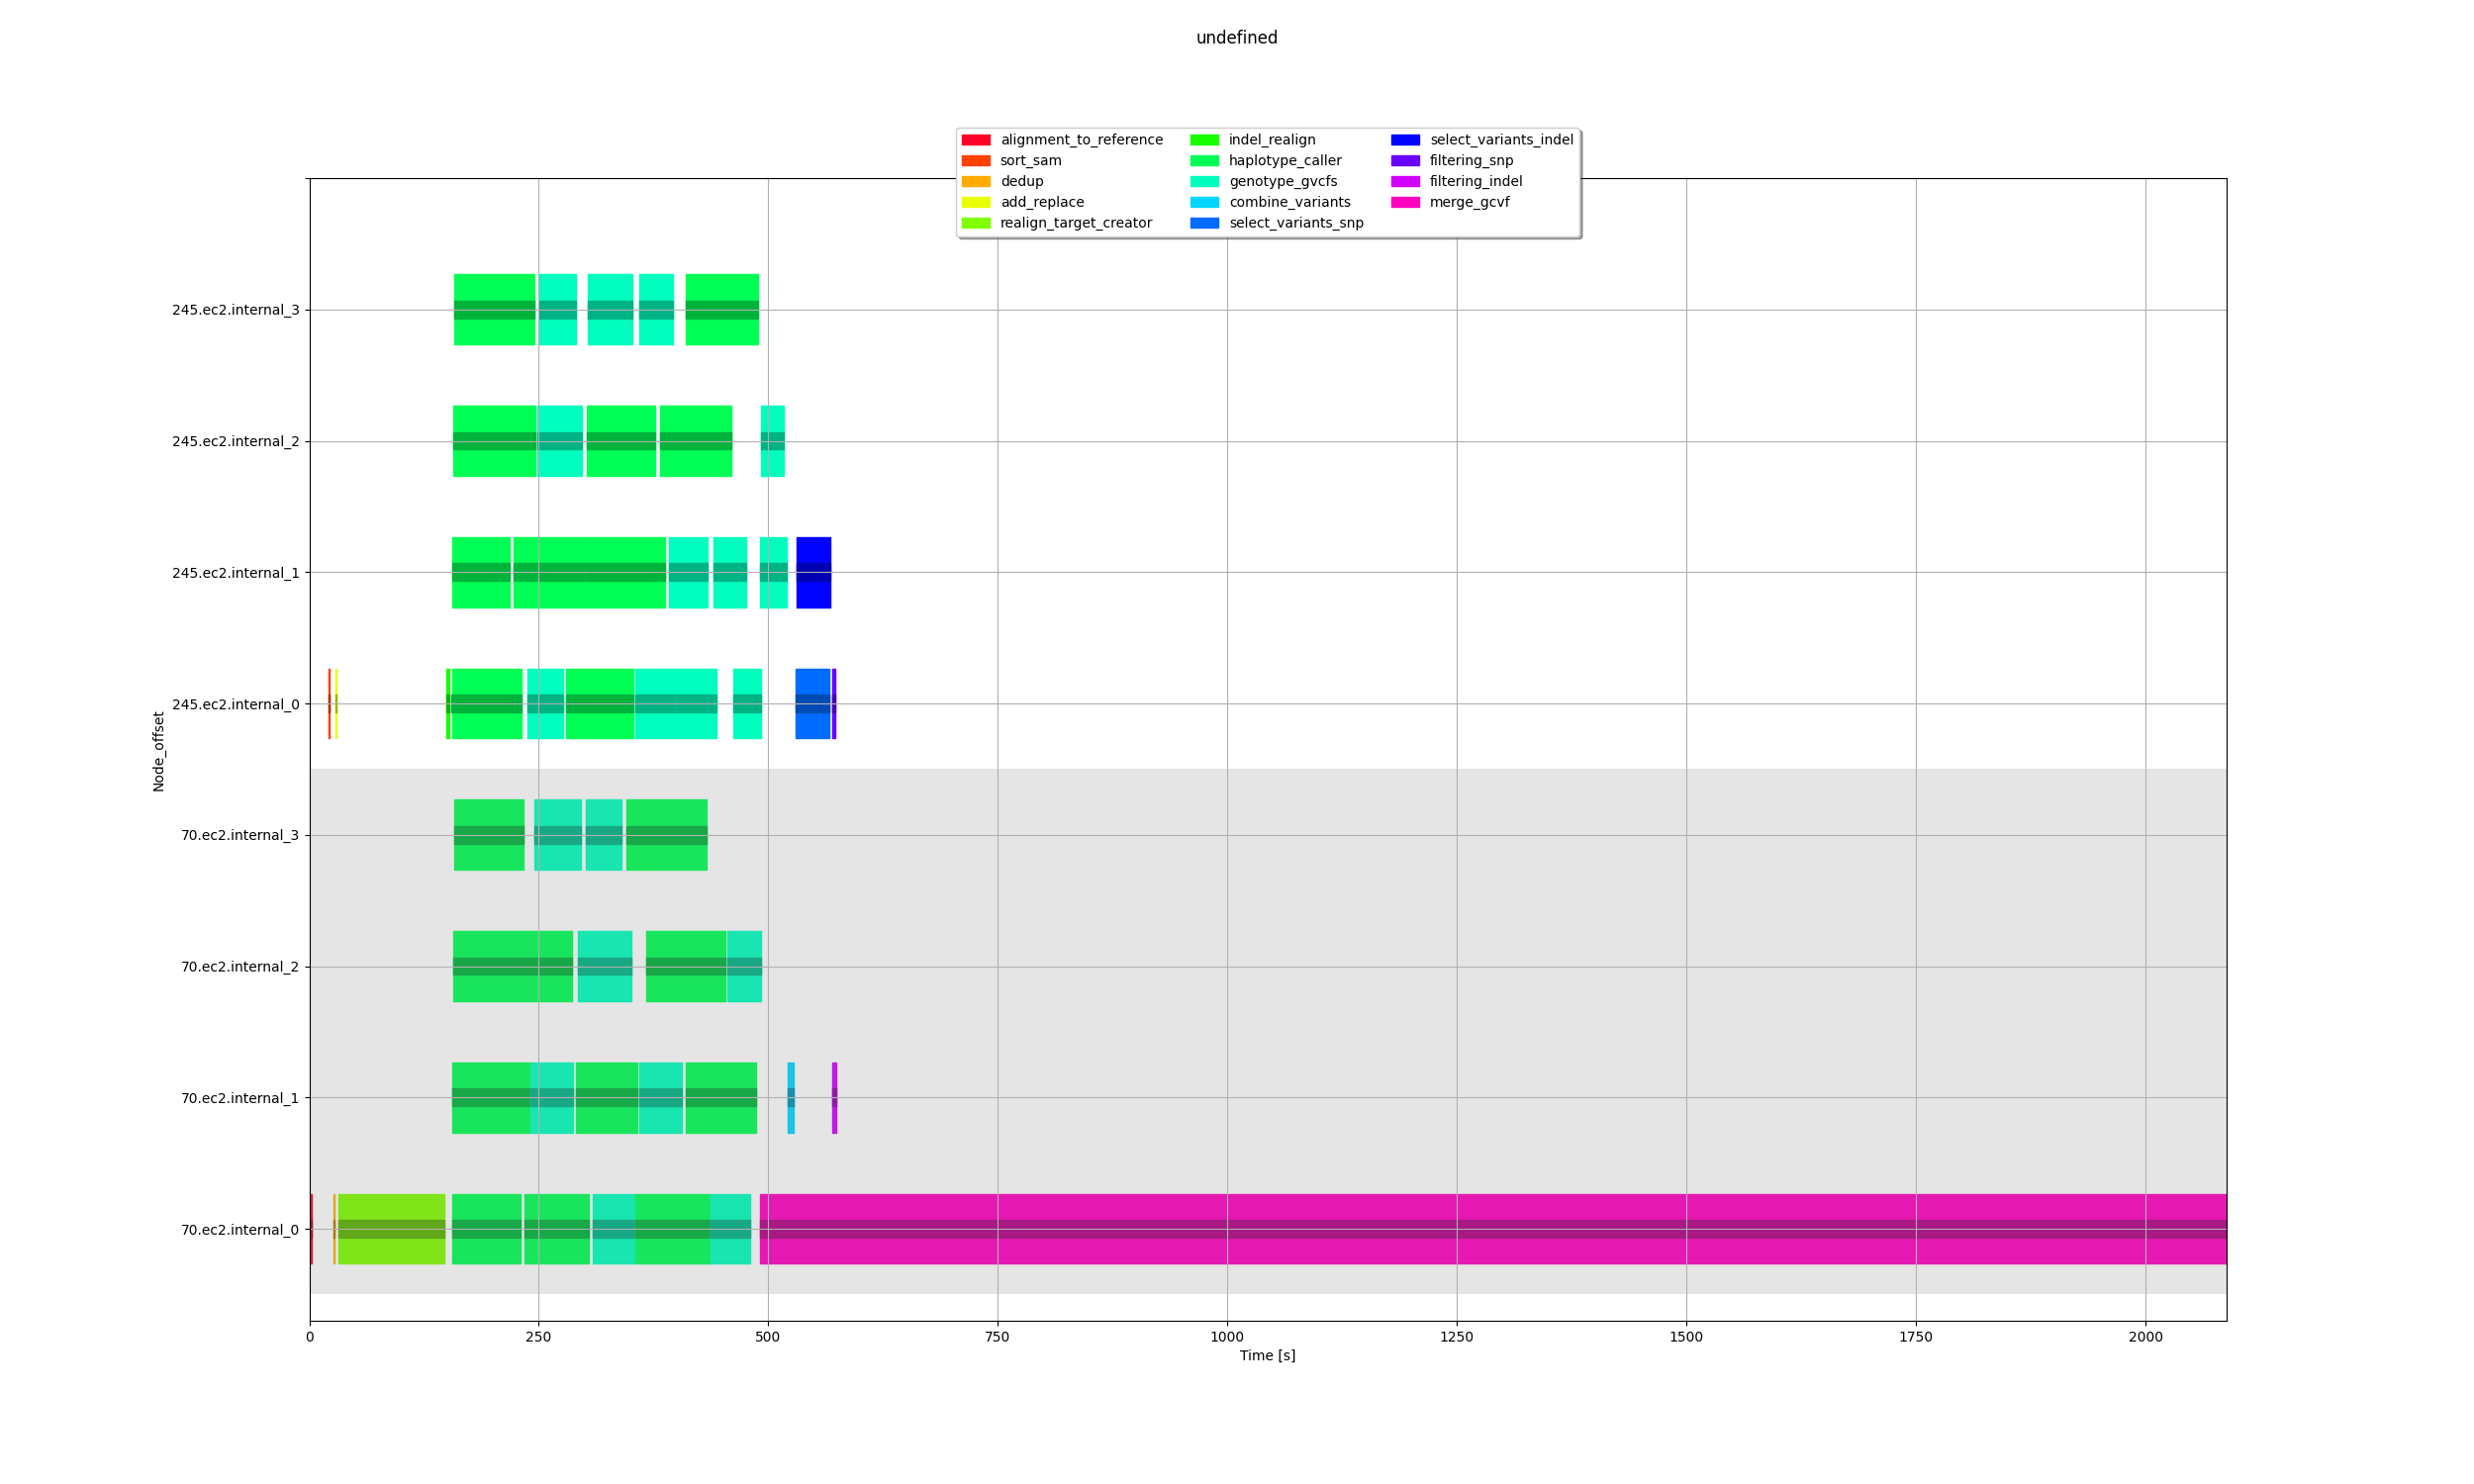
\includegraphics[width=1\linewidth]{figures/6-1-soykb-empty.png}
% %%
% \caption[Trace for sole kube-scheduler schedule on SoyKB]{Trace for sole kube-scheduler schedule on SoyKB.}
% \label{fig:evaluation:sched:soykb:empty}
% \end{figure}
% %%%%%%%
% \begin{figure}[H]
% \begin{subfigure}{1\textwidth}
% \centering
% 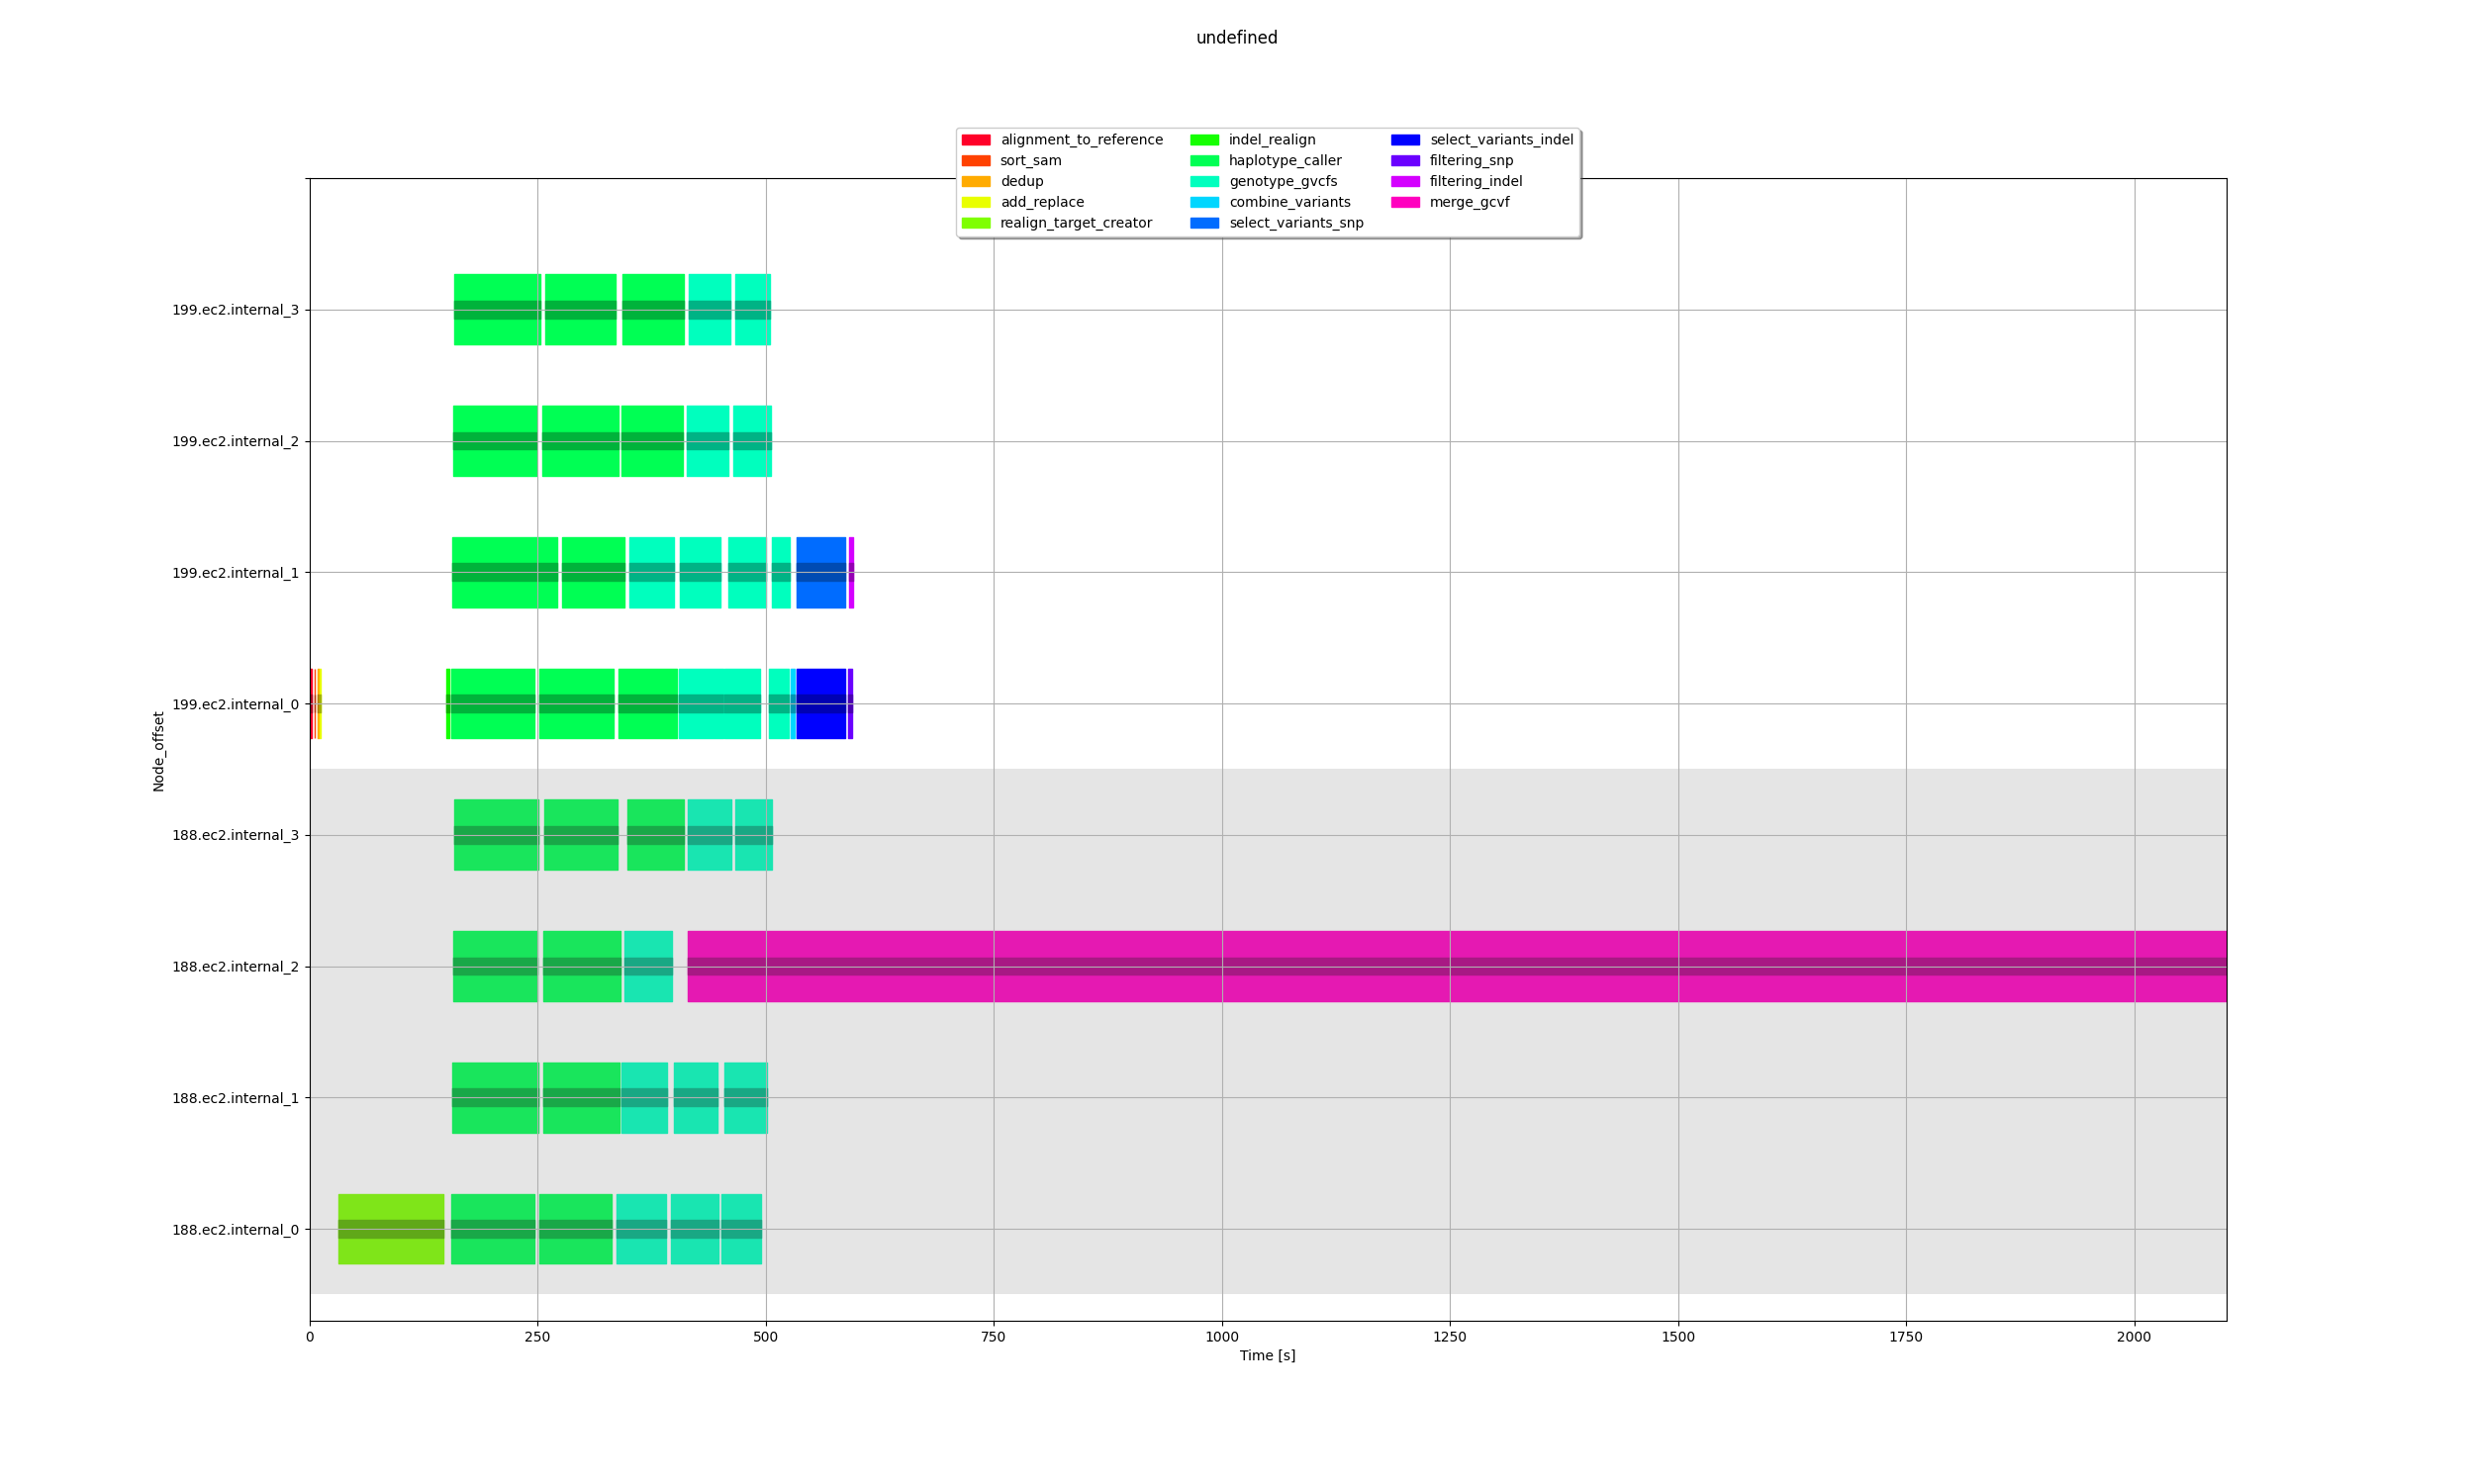
\includegraphics[width=1\linewidth]{figures/6-1-soykb-heft.png}
% \caption[Execution trace with HEFT scheduler plugin on SoyKB]{HEFT}
% \label{fig:evaluation:sched:soykb:heft}
% \end{subfigure}
% \begin{subfigure}{1\textwidth}
% \centering
% 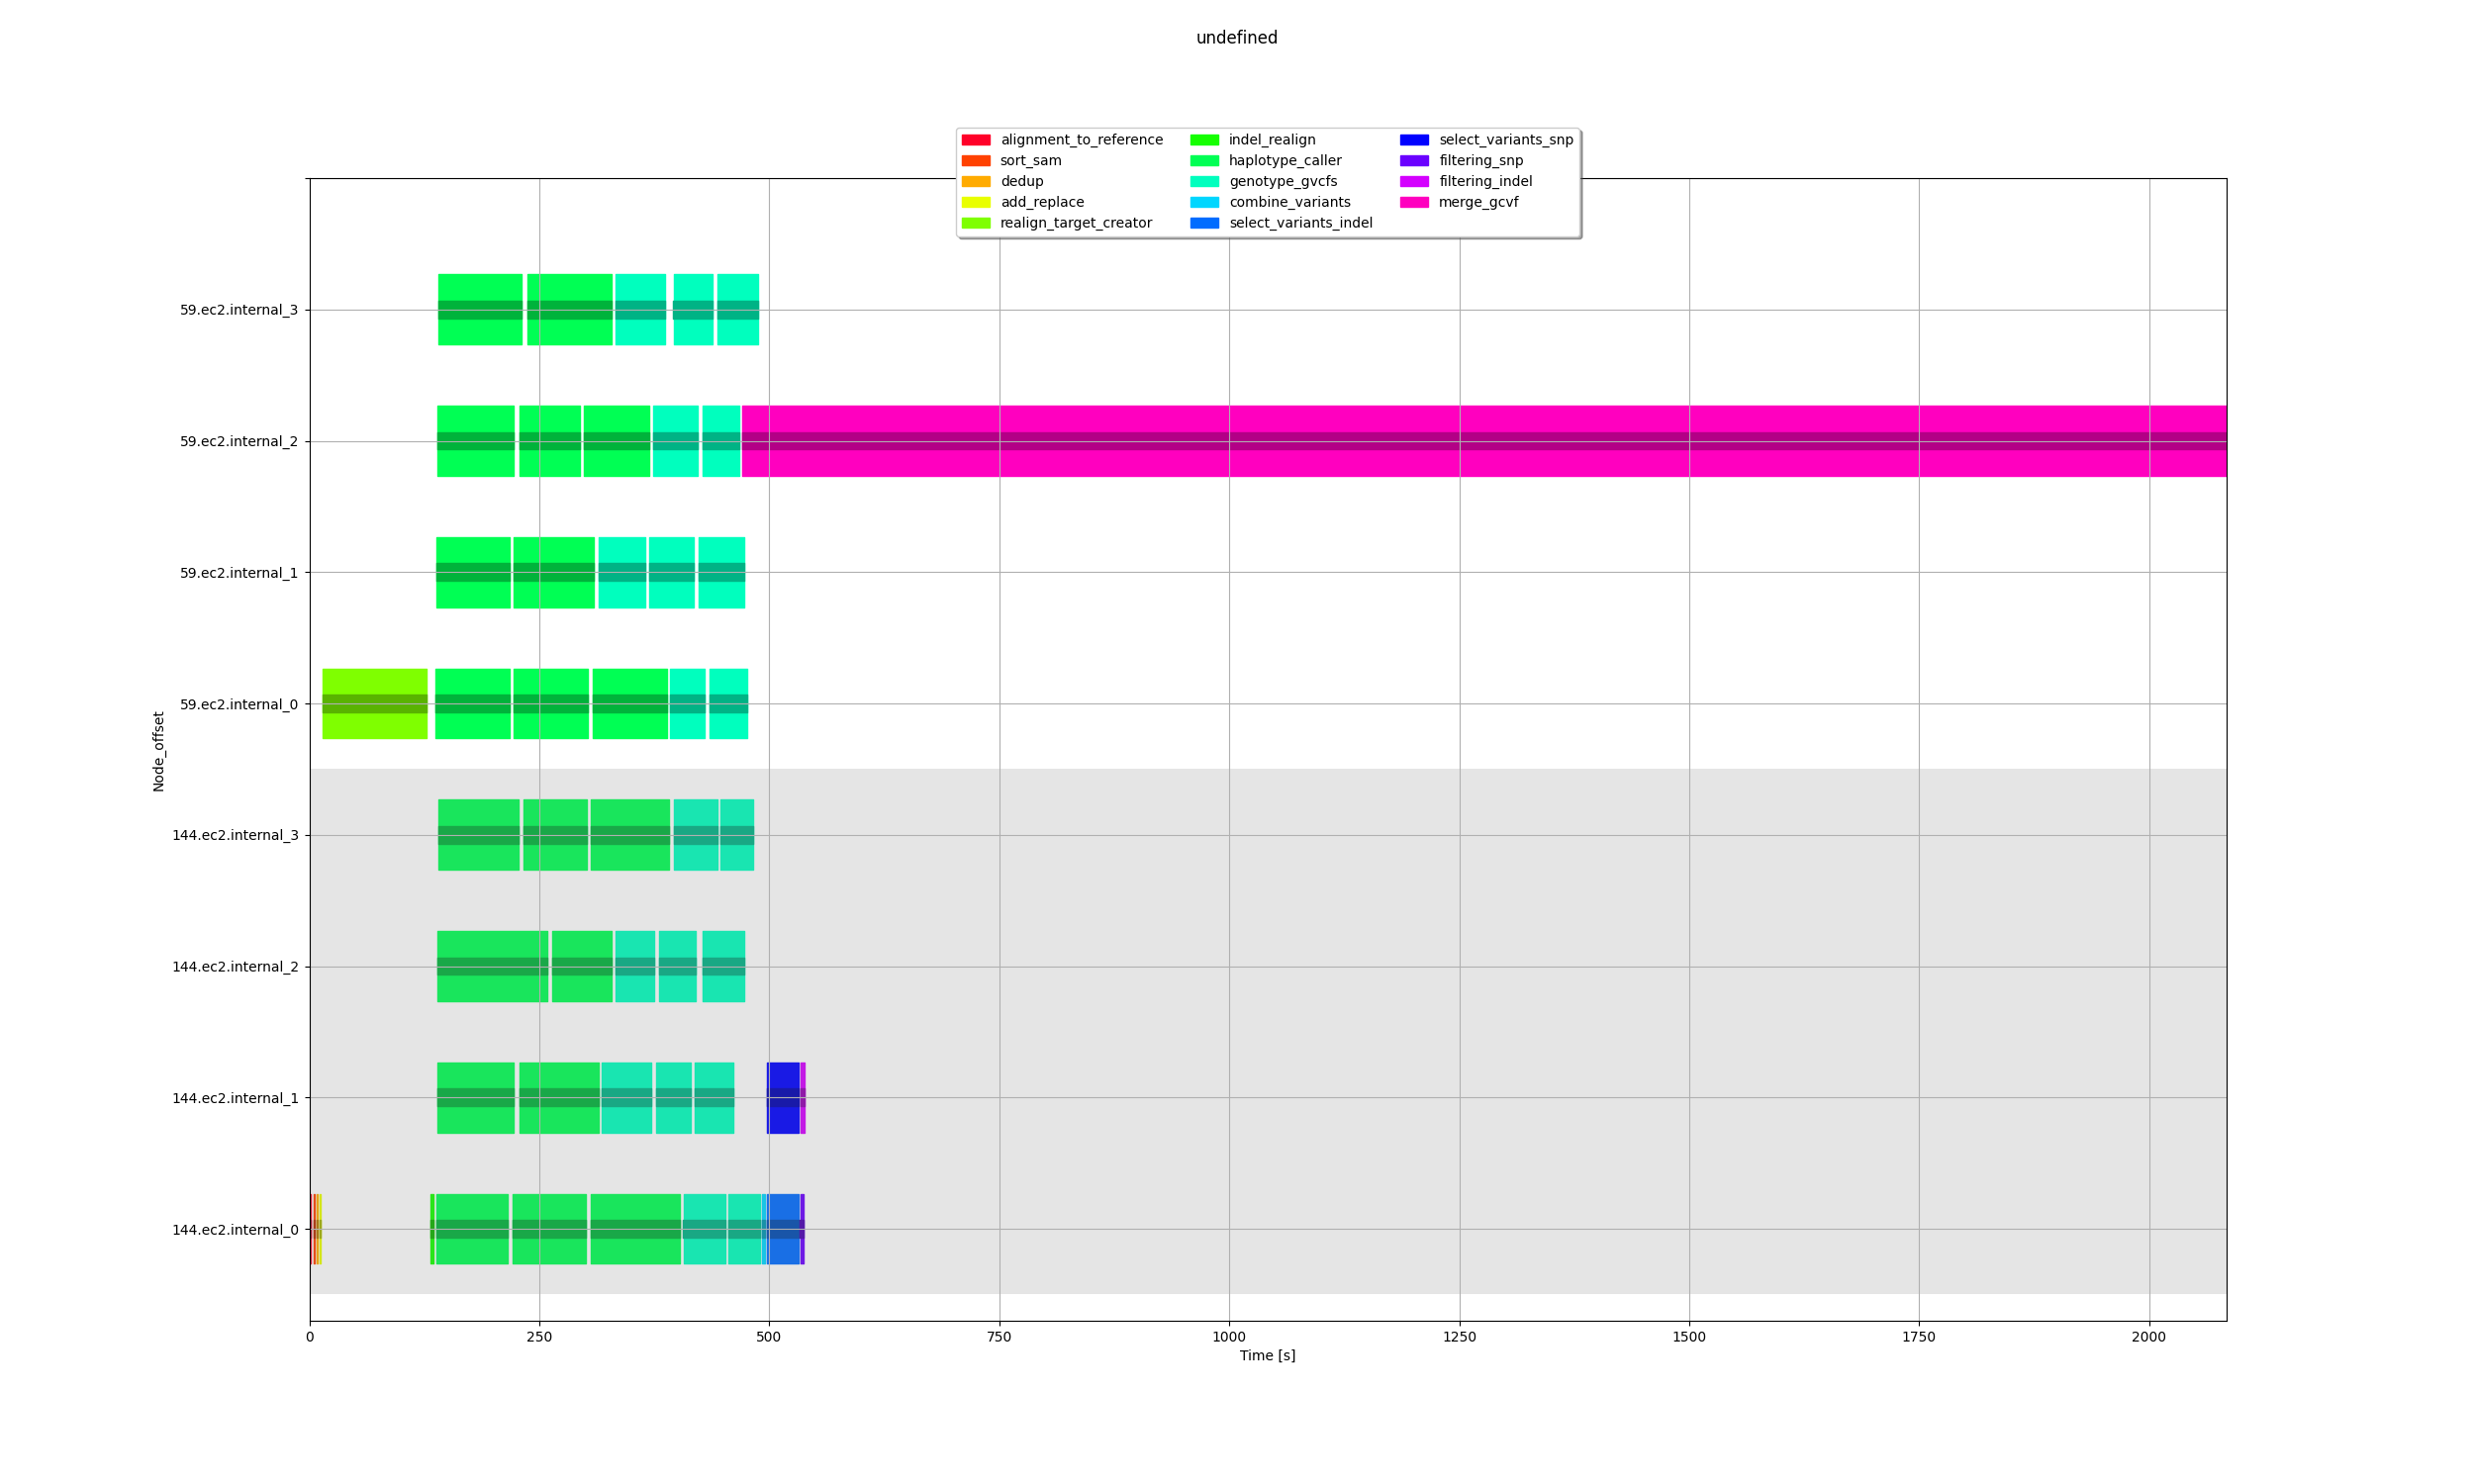
\includegraphics[width=1\linewidth]{figures/6-1-soykb-peft.png}
% \caption[Execution trace with PEFT scheduler plugin on SoyKB]{PEFT}
% \label{fig:evaluation:sched:soykb:peft}
% \end{subfigure}
% \centering
% %%
% \caption[Execution traces with scheduler plugin on SoyKB]{Execution traces with scheduler plugin on SoyKB.}
% %%
% \medskip
% \begin{minipage}{0.75\textwidth}
% {\footnotesize Blah blah \par}
% \end{minipage}
% %%
% \label{fig:evaluation:sched:soykb:plugin}
% \end{figure}

%%%%%%%

\begin{figure}[H]
\begin{subfigure}{0.75\textwidth}
\centering
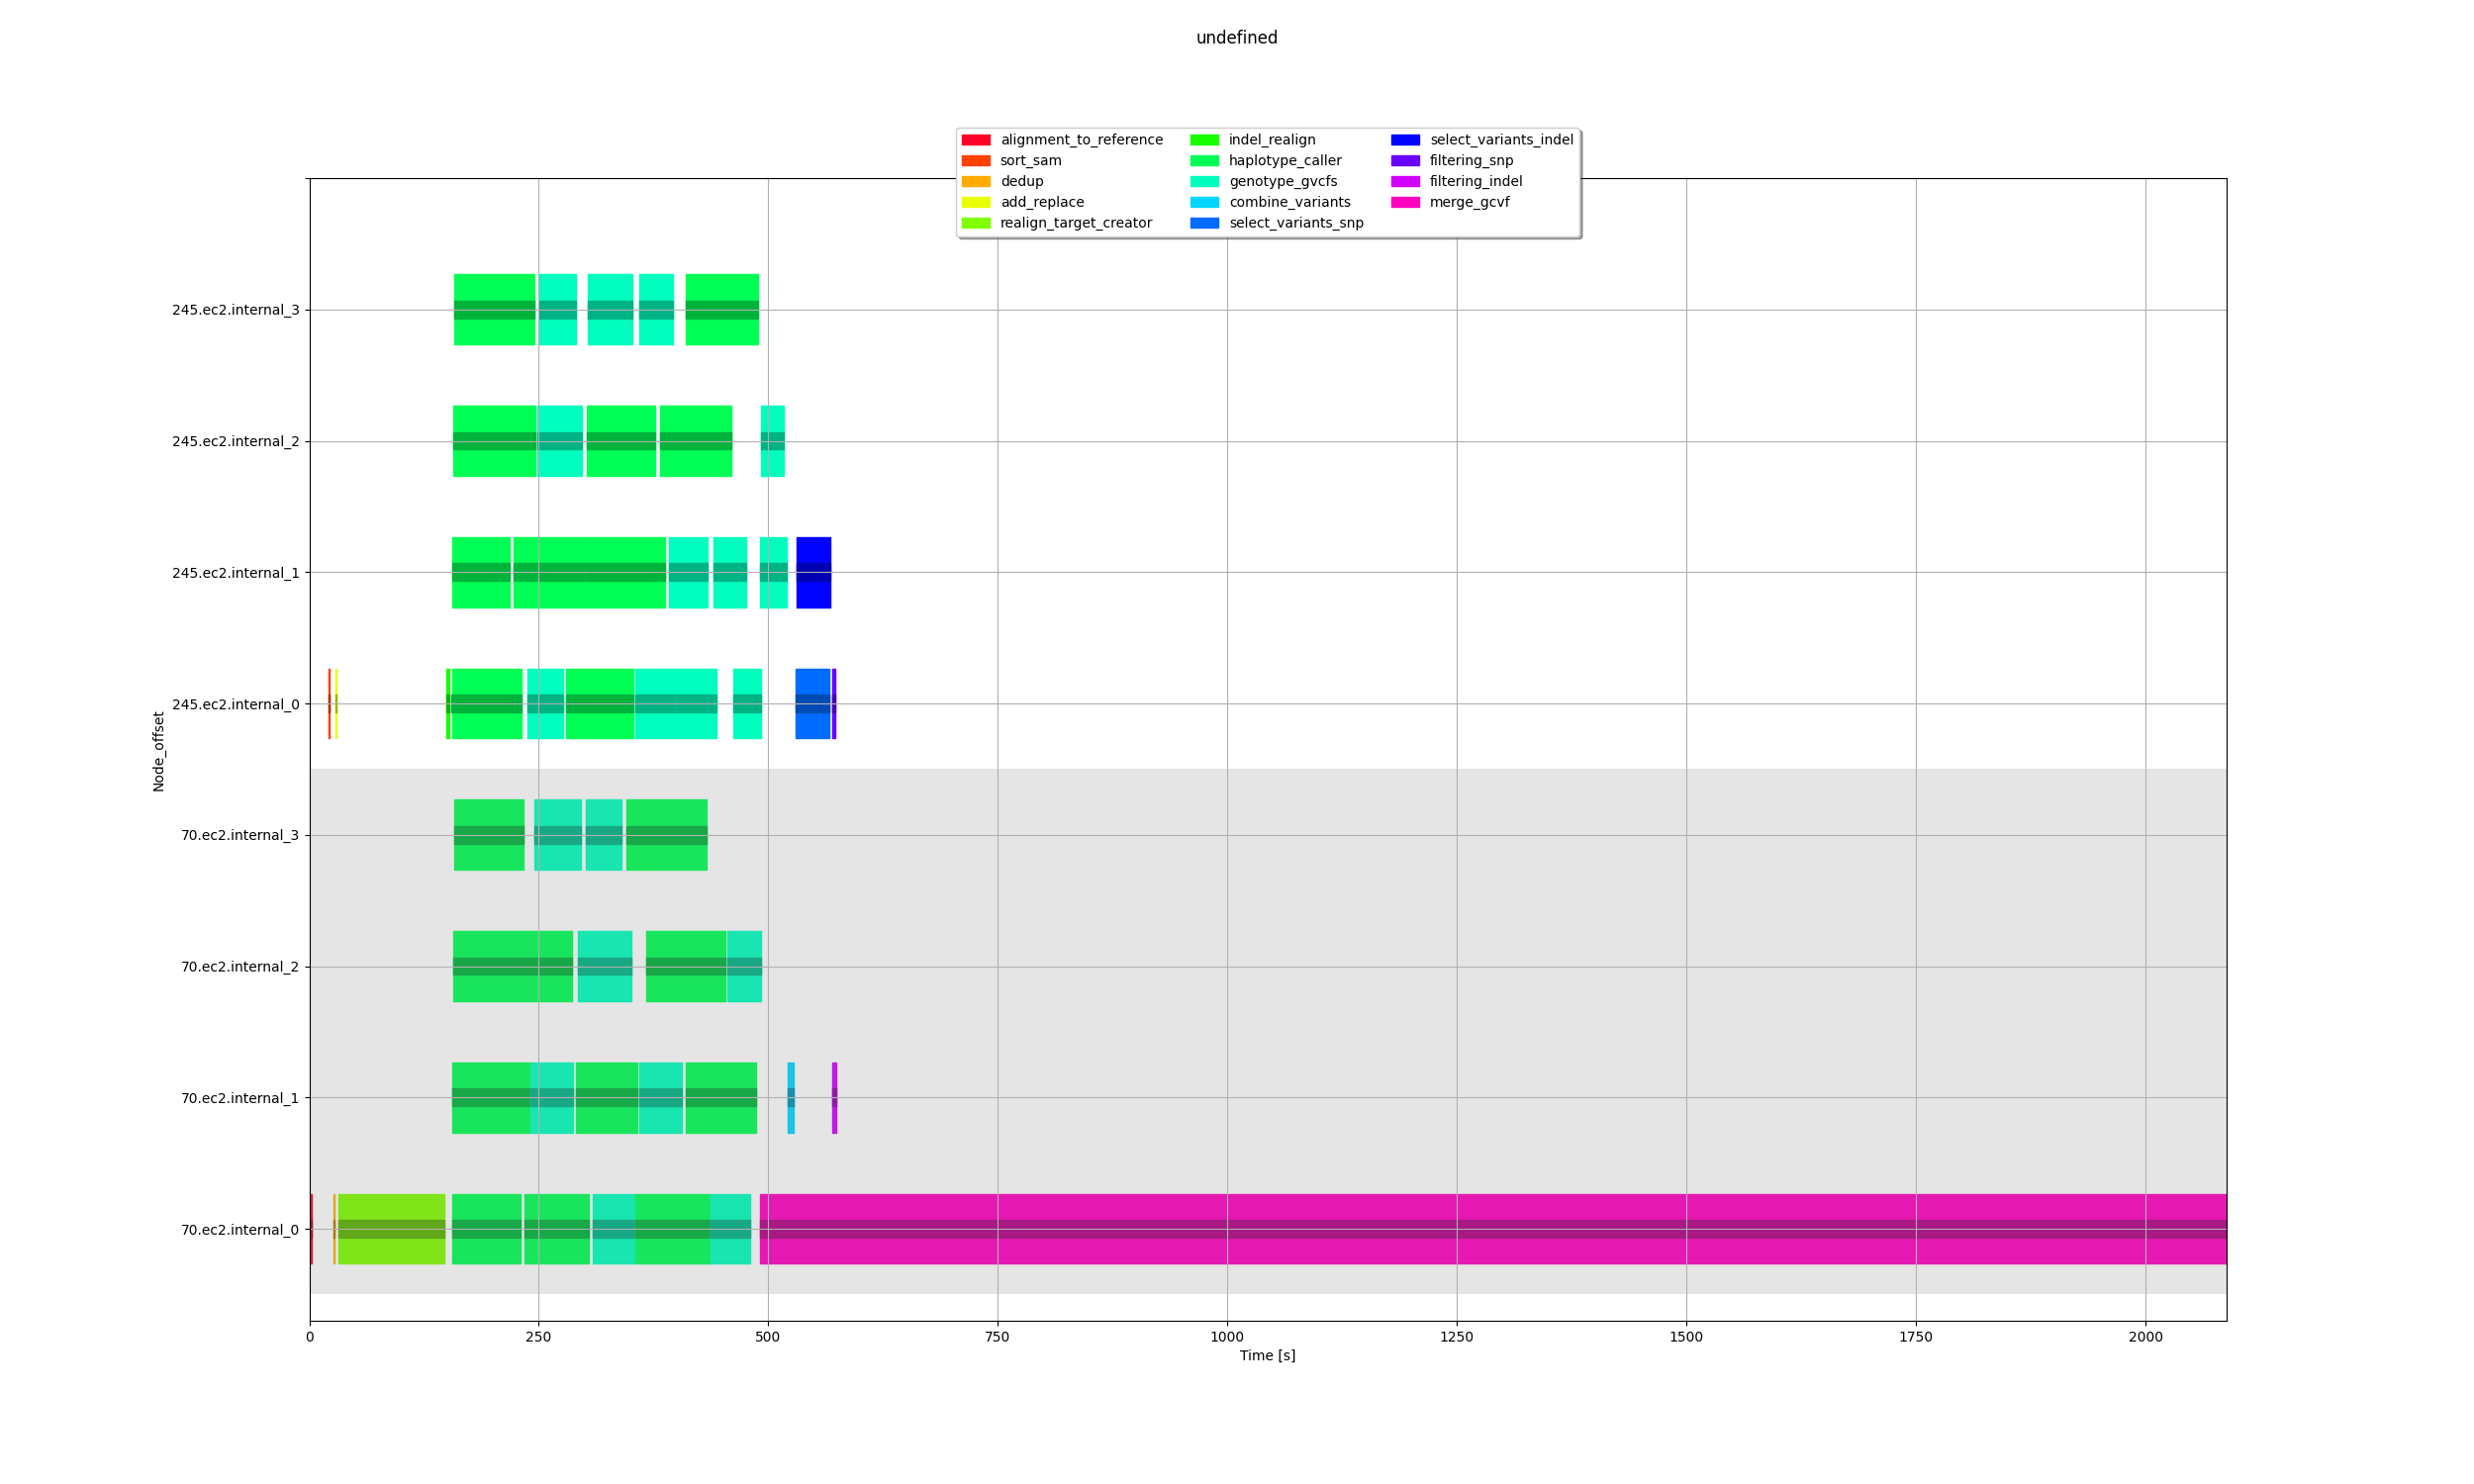
\includegraphics[width=1\linewidth]{figures/6-1-soykb-empty.png}
\caption[Selected example execution trace for SoyKB workflow without static scheduling]{w/o scheduler plugin}
\label{fig:evaluation:sched:soykb:empty}
\end{subfigure}
\begin{subfigure}{0.75\textwidth}
\centering
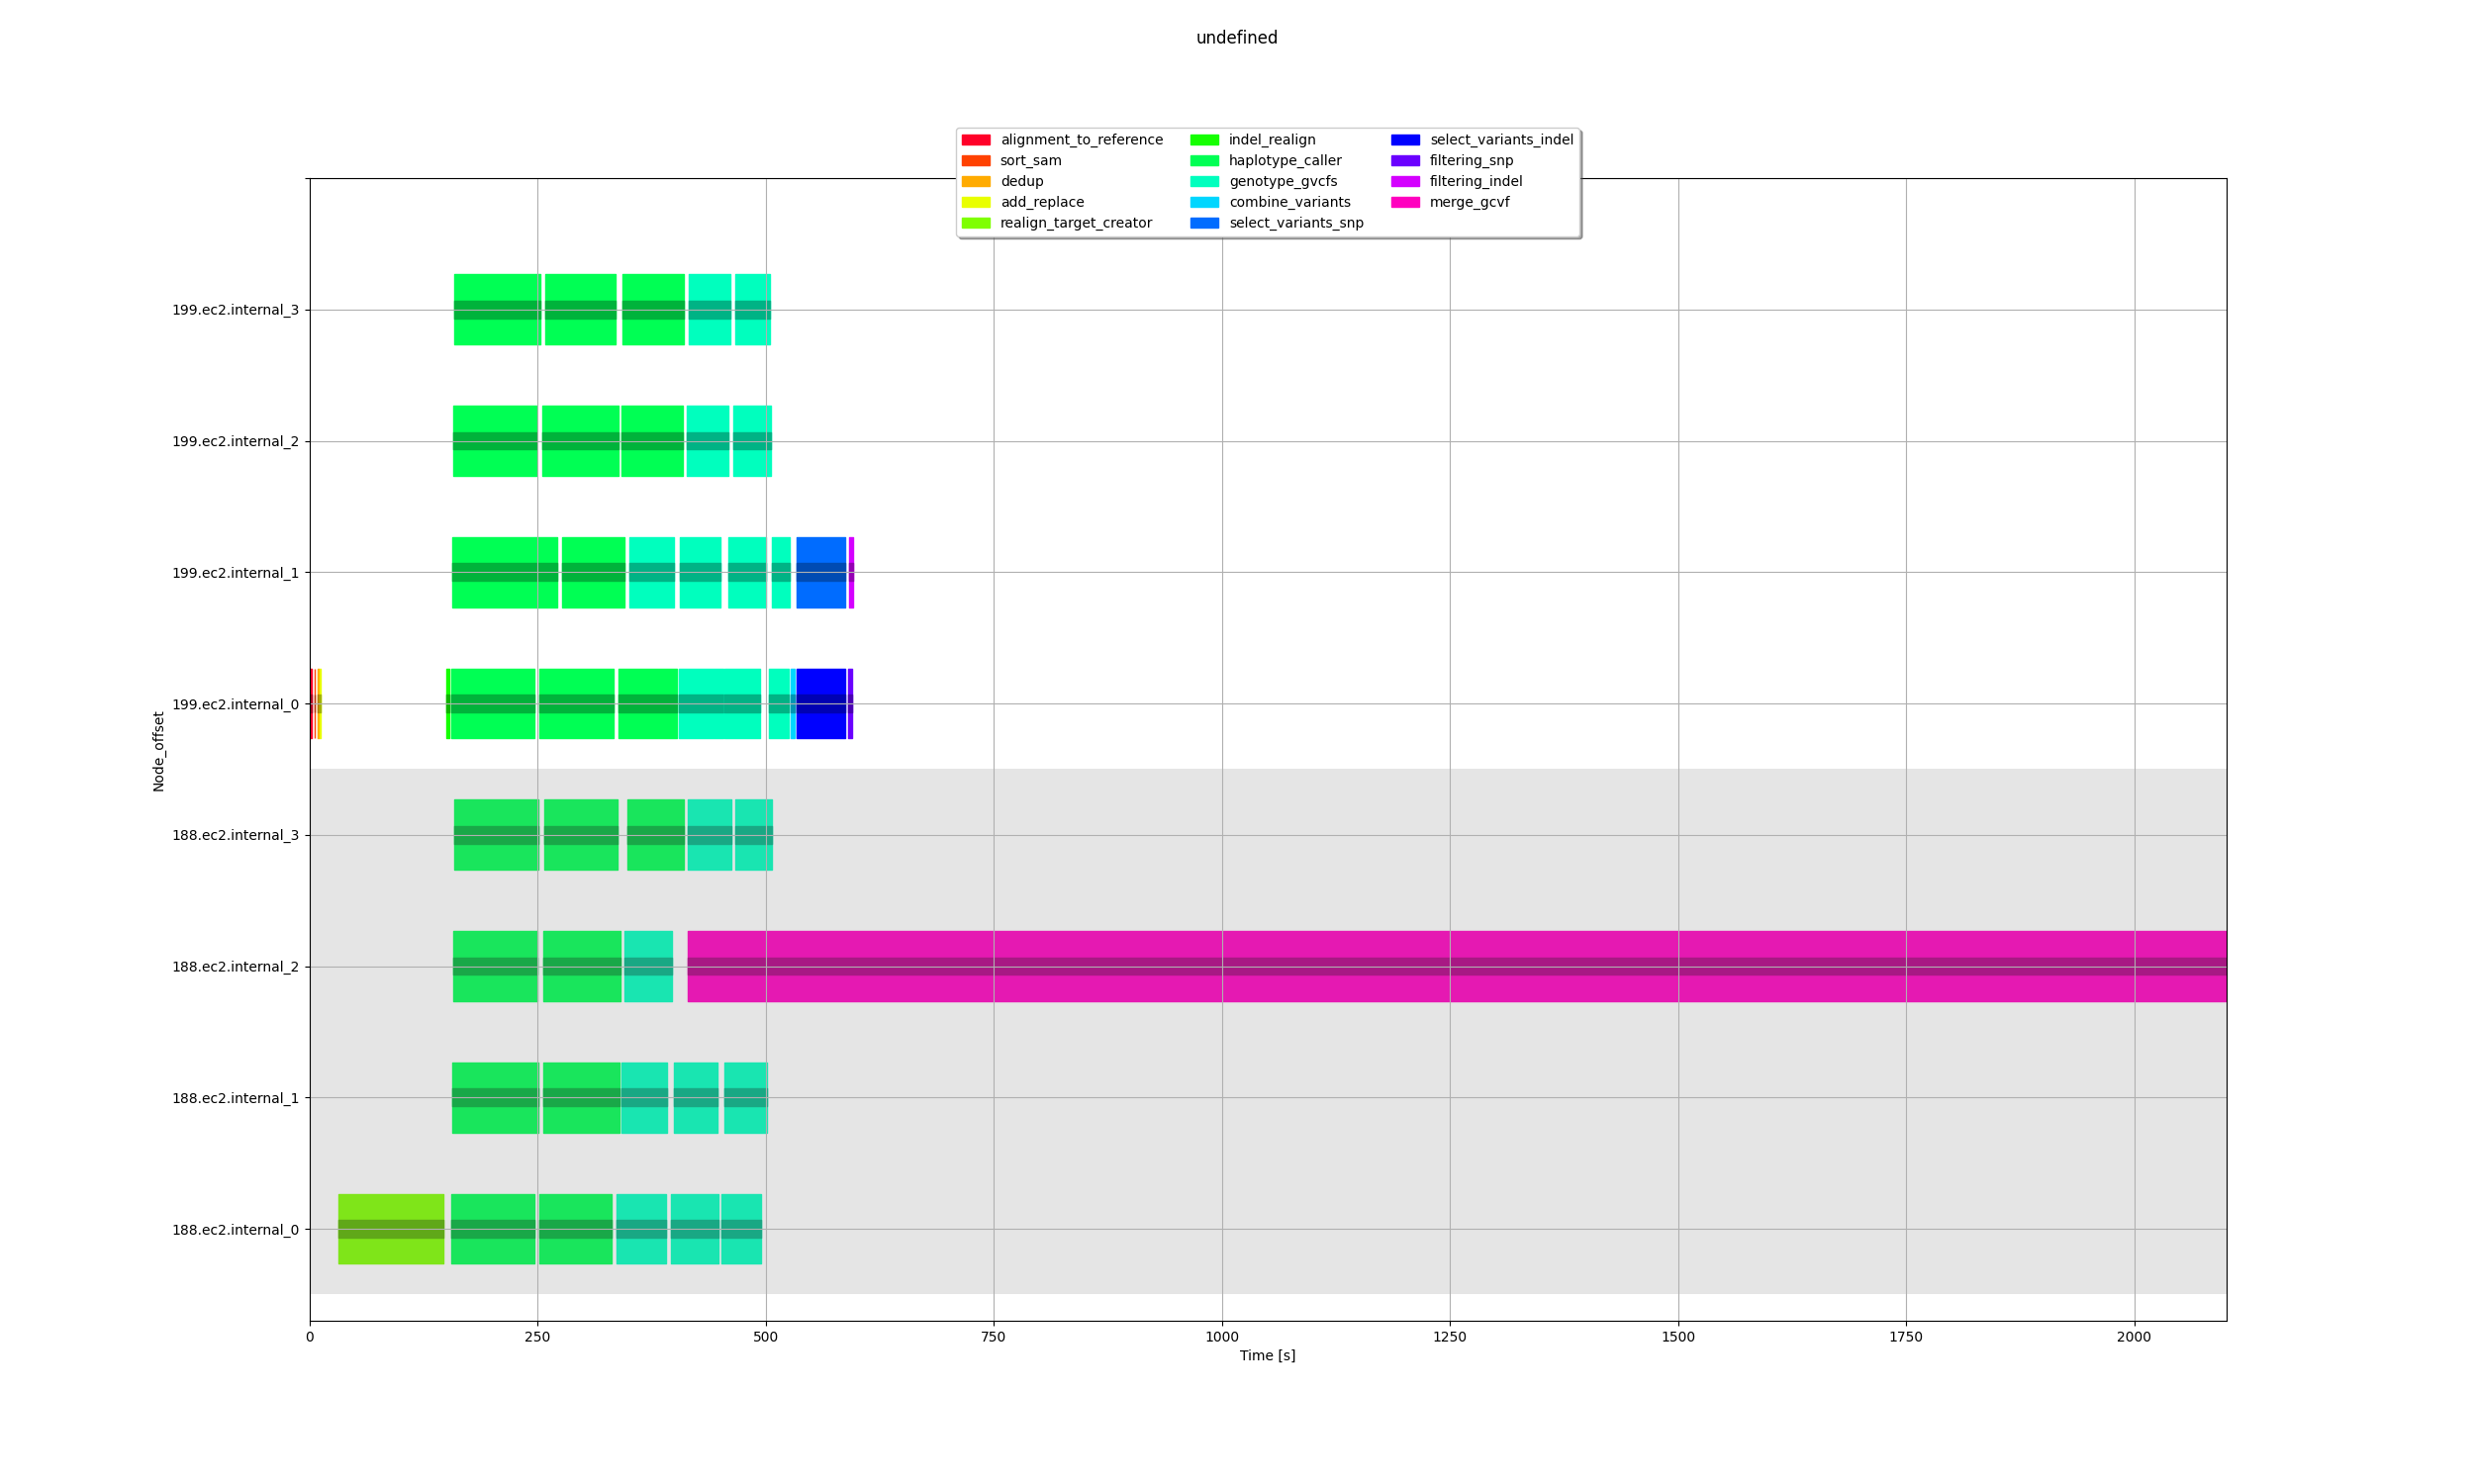
\includegraphics[width=1\linewidth]{figures/6-1-soykb-heft.png}
\caption[Selected example execution traces for SoyKB workflow with HEFT]{HEFT}
\label{fig:evaluation:sched:soykb:heft}
\end{subfigure}
\begin{subfigure}{0.75\textwidth}
\centering
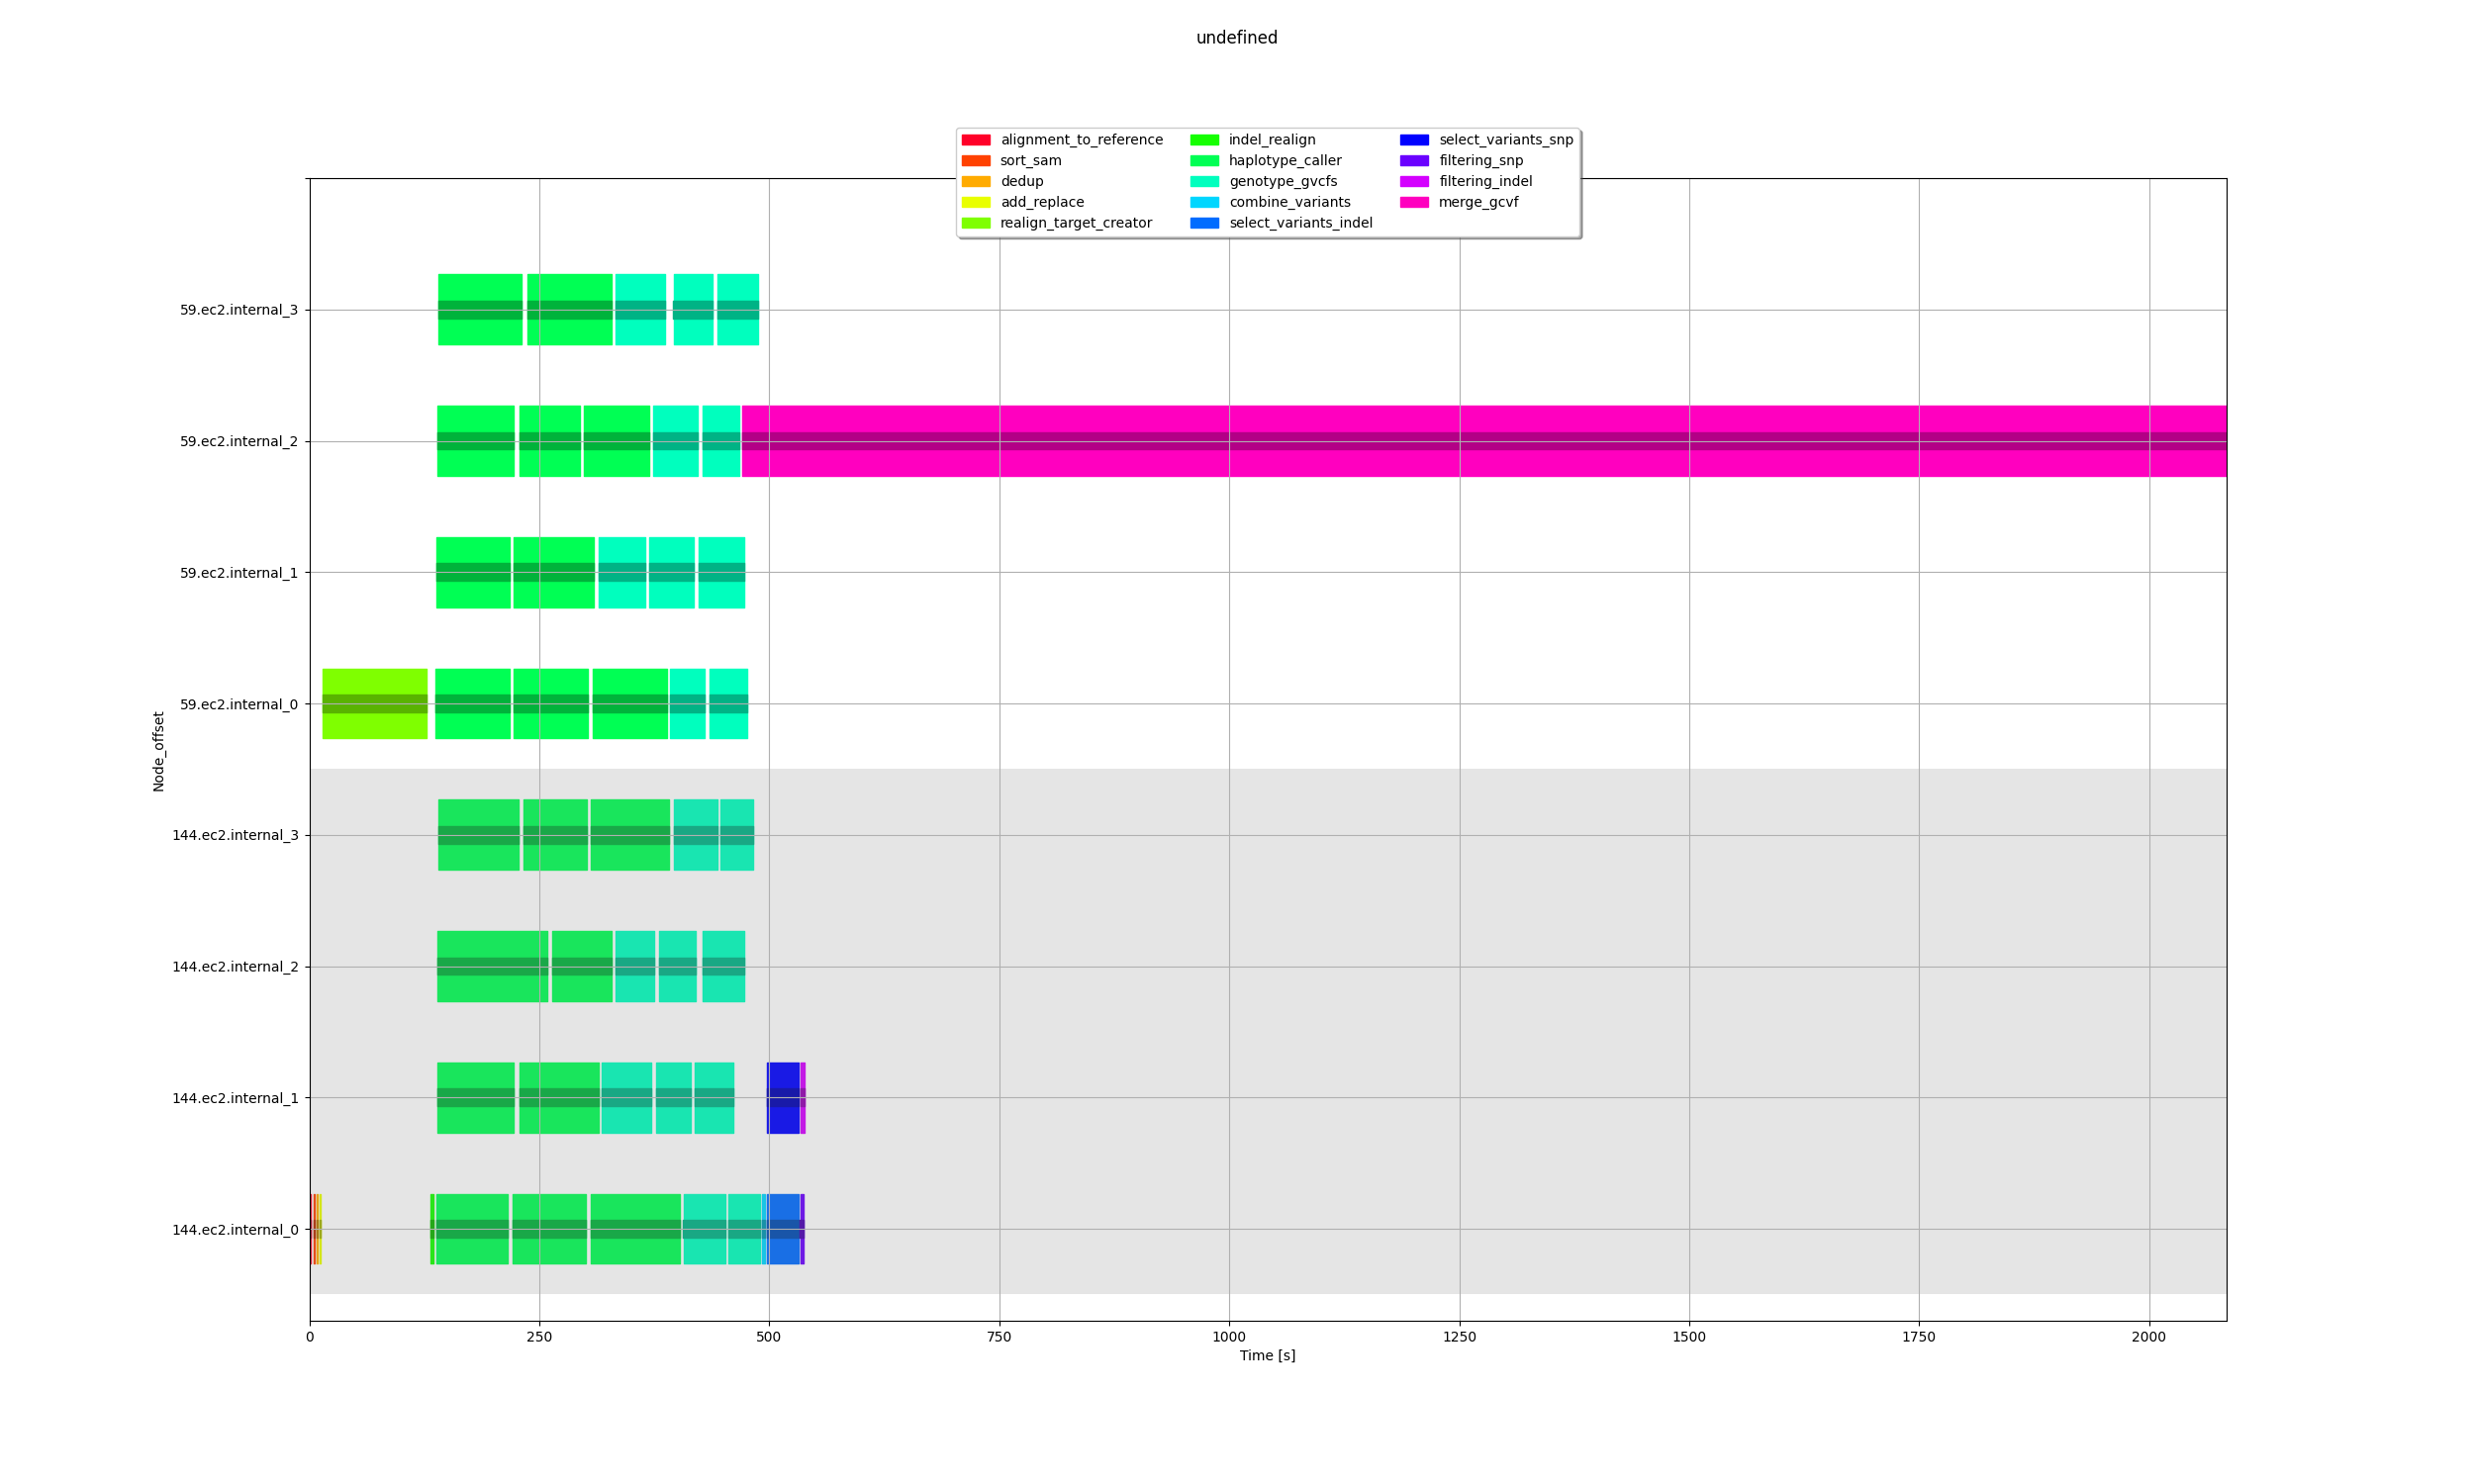
\includegraphics[width=1\linewidth]{figures/6-1-soykb-peft.png}
\caption[Selected example execution traces for SoyKB workflow with PEFT]{PEFT}
\label{fig:evaluation:sched:soykb:peft}
\end{subfigure}
\centering
%%
\caption[Selected example execution traces for SoyKB workflow]{Selected example execution traces for SoyKB workflow.}
%%
% \medskip
% \begin{minipage}{0.75\textwidth}
% % {\footnotesize Blah blah aaaaa aaaaa aaaaaaaaaaaaaaa aaaaa aaaaa aaaaaaaaaa aaaaaaaaaa aaaaa aaaaa aaaaa aaaaa aaaaa aaaaa aaaaa v v aaaaa aaaaa aaaaa aaaaa aaaaa \par}
% \end{minipage}
% \medskip
%%
\label{fig:evaluation:sched:soykb}
\end{figure}

%%%%%%%

%%%%
% Tabelka z metrykami - SoyKB
\begin{table}[H]
    \centering
    \begin{tabular}{|c|c|c|c|c|}
    \cline{1-5}
        \multirow{2}{*}{Approach} 
        &
        \multicolumn{4}{|c|}{Metrics} \\
    \cline{2-5}
        & Makespan & Slowdown & SLR & CO \\
    \cline{1-5}
        kube-scheduler & 2191 & 2.2 & 1.14 & 249 \\
    \cline{1-5}
        HEFT + kube-scheduler & 2089 & 2.8 & 1.24 & 237  \\
    \cline{1-5}
        PEFT + kube-scheduler & 2115 & 2.6 & 1.13 & 246 \\
    \cline{1-5}
    \end{tabular}
    \caption{Average metric results for SoyKB}
    \label{tab:metrics-sched-soykb}
\end{table}
%%%%


Based on the makespan values, using static scheduling for SoyKB allows to shorten the workflow execution time by about 4\%.
This comes at the cost of higher job slowdown, which likely is a result of enforcing an execution of a specific schedule.
In this case, HEFT schedule is slightly more effective than PEFT one, however the reasons for that are not entirely clear, at least not from a metric perspective.
Following the execution traces, it seems to be possible that with HEFT schedule (\cref{fig:evaluation:sched:soykb:heft}) the longest task manages to start a bit earlier than with the other solutions, and thus HEFT achieves slightly better job parallelization, shortening the overall run time.
As for the improvement over the approach without scheduling, it likely comes from choosing a better suited machine to execute the task on, based on the calculated schedule.



On the other hand, the case with Montage workflow provides results (\cref{tab:metrics-sched-m025}) supporting claims contradictory to the conclusions drawn from SoyKB execution.
Here, the default solution without scheduler plugin performs much better on a Montage workflow, with over 18\% shorter makespan, a few times lower job slowdown, and SLR closer to the optimal compared to any other approach.



% The differences

% scattered, parallelized, 

% 
% Popatrz na obrazki montage - sa na jednym CPU i dlatego sie psuje
%

%%%%
% Tabelka z metrykami - Montage-0.25
\medskip
\begin{table}[H]
    \centering
    \begin{tabular}{|c|c|c|c|c|}
    \cline{1-5}
        \multirow{2}{*}{Approach} 
        &
        \multicolumn{4}{|c|}{Metrics} \\
    \cline{2-5}
        & Makespan & Slowdown & SLR & CO \\
    \cline{1-5}
        kube-scheduler & 821 & 474 & 22.3 & 4511 \\
    \cline{1-5}
        HEFT + kube-scheduler & 995 & 2278 & 30.8 & 4000 \\
    \cline{1-5}
        PEFT + kube-scheduler & 972 & 1194 & 29.7 & 3729 \\
    \cline{1-5}
    \end{tabular}
    \caption{Average metric results for Montage2-v0.25}
    \label{tab:metrics-sched-m025}
\end{table}
%%%%

With the execution traces presented in \cref{fig:evaluation:sched:m025:plugin} it is easier to find a possible hypothesis for such incoherent results across different applications.
As most of the tasks are shown to be executed on the same CPU, it could indicate that there is a problem with proper task parallelization during Montage workflow execution.
Most of the tasks (mainly \emph{mDiffFit} and \emph{mBackground}) take so little time to complete that their container lifespan is short enough to possibly overload the Kubernetes cluster with constant pod lifecycle management requests.
\begin{figure}[H]
%%
    \begin{subfigure}{1\textwidth}
        \centering
        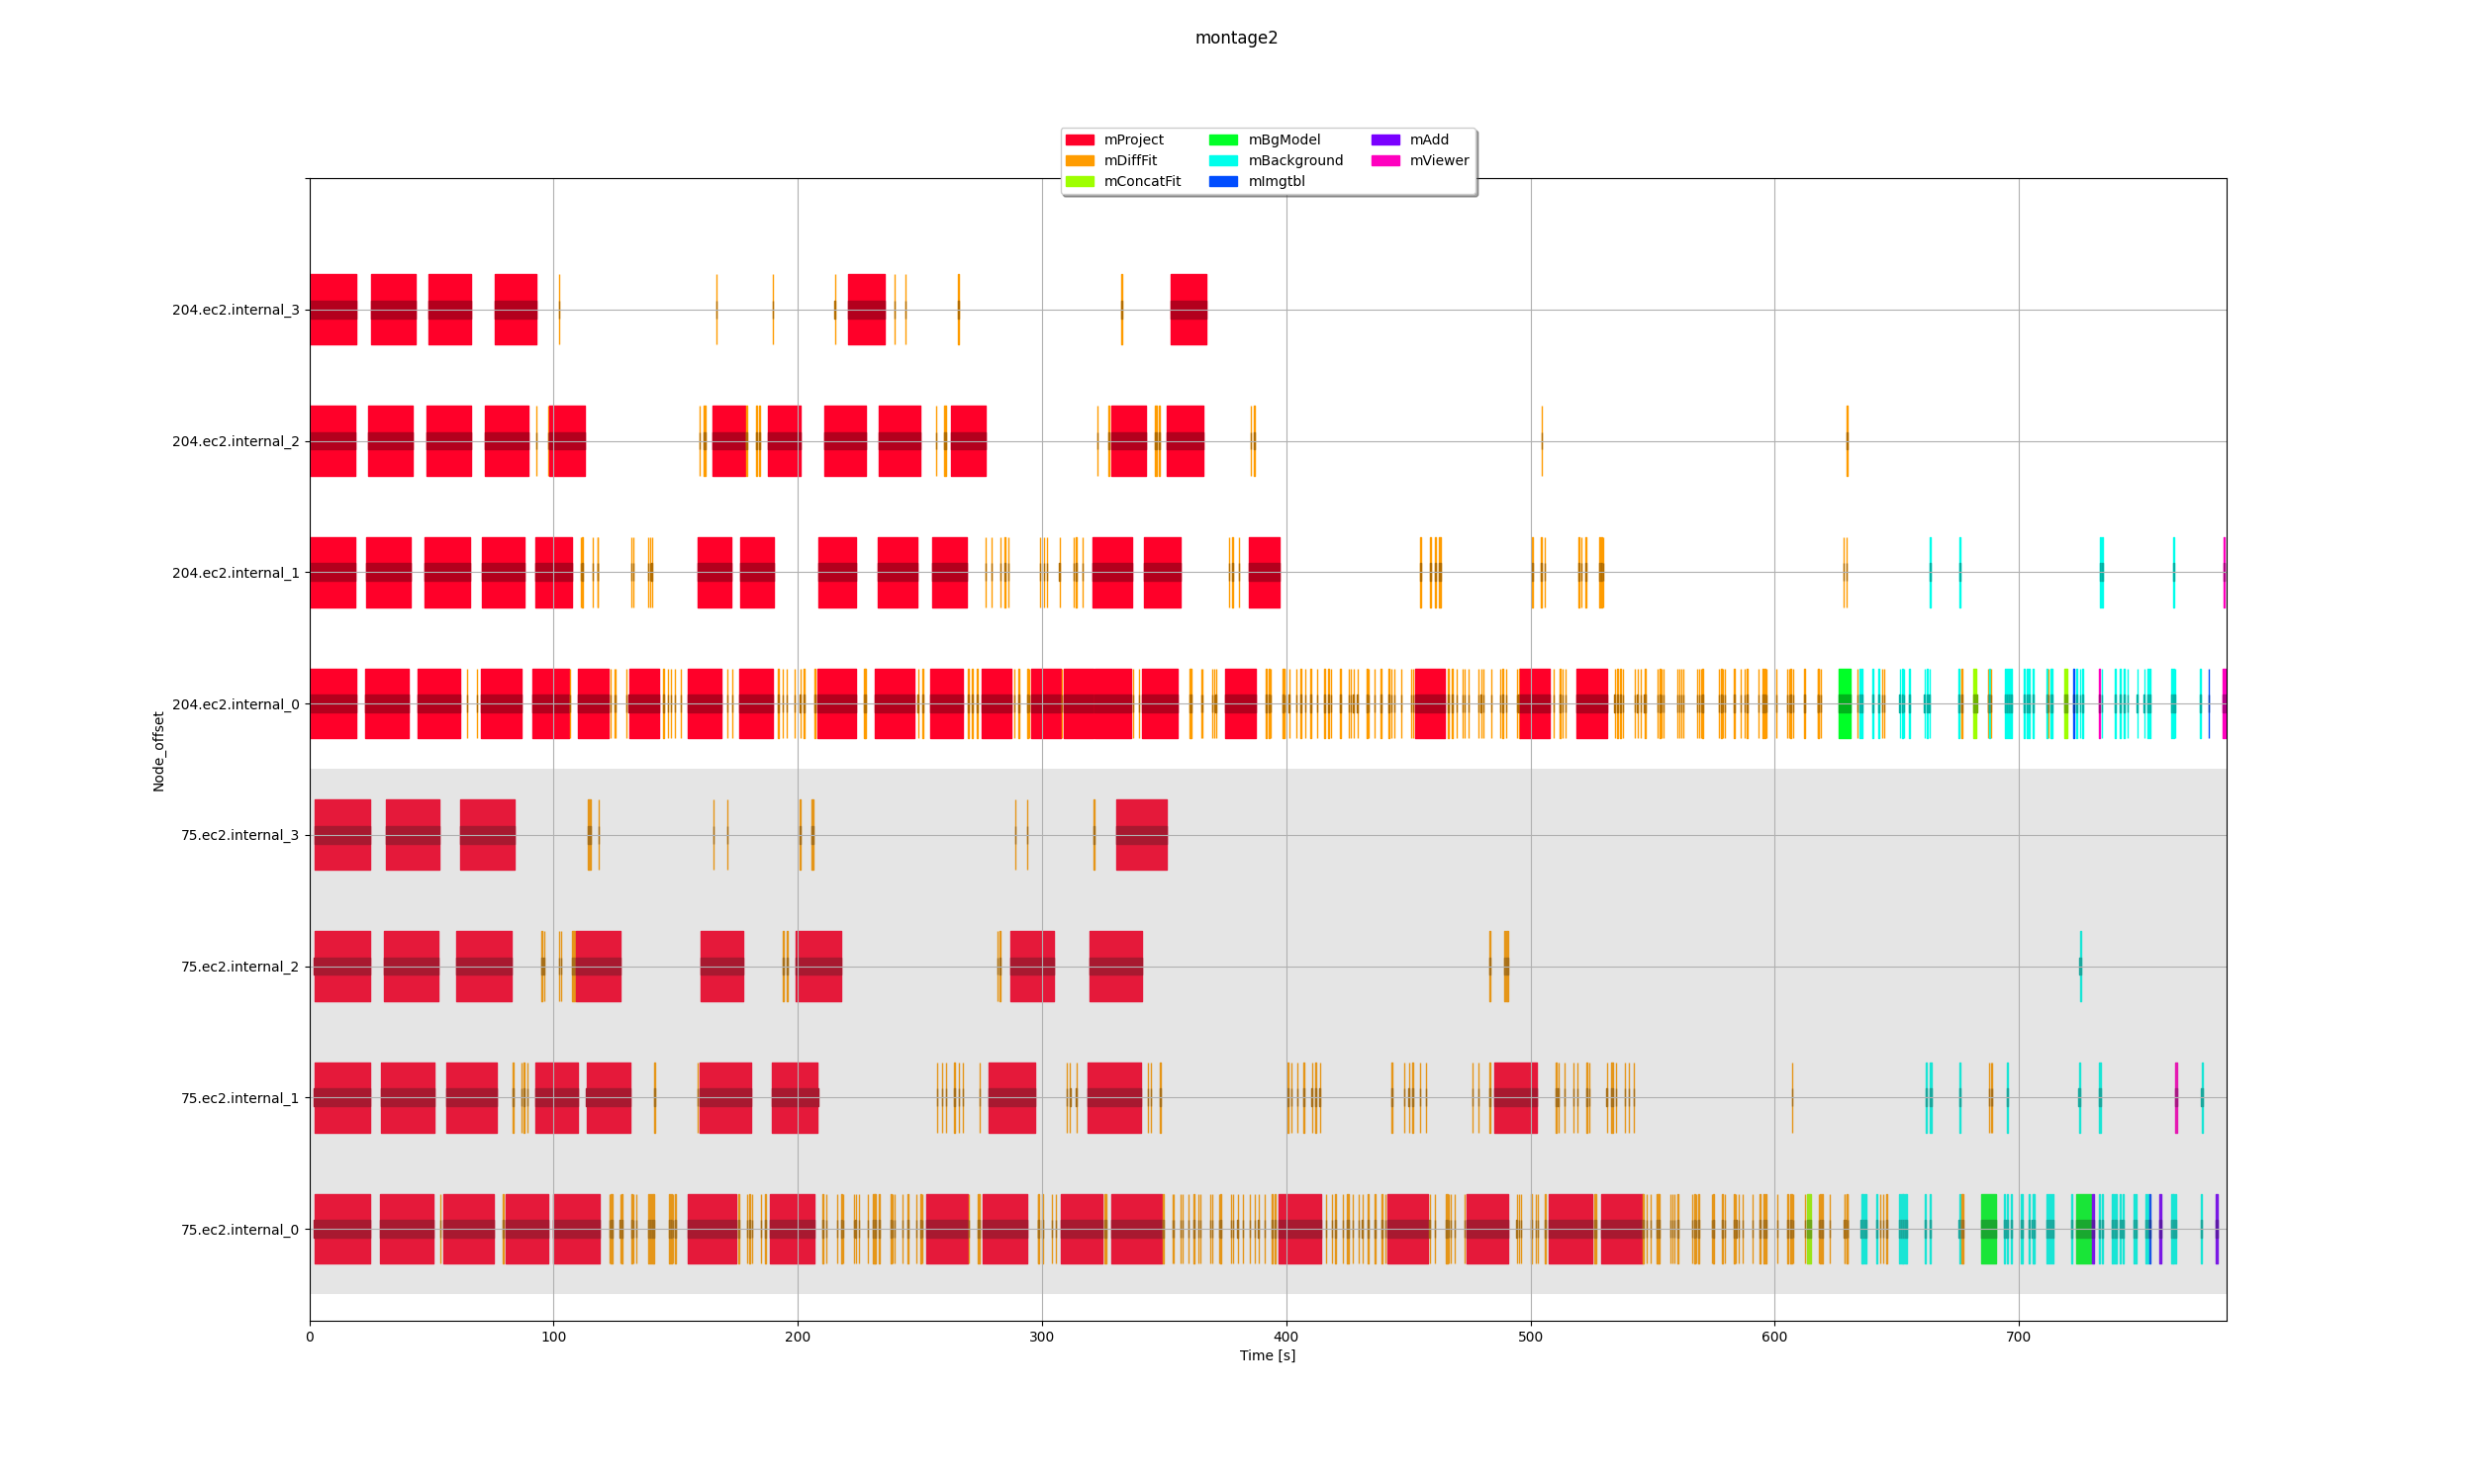
\includegraphics[width=0.75\linewidth]{figures/6-1-m0.25-empty.png}
        \caption[Selected example execution trace for Montage2-v0.25 workflow without static scheduling]{w/o scheduler plugin}
        \label{fig:evaluation:sched:m025:em}
    \end{subfigure}
%%
    \begin{subfigure}{1\textwidth}
        \centering
        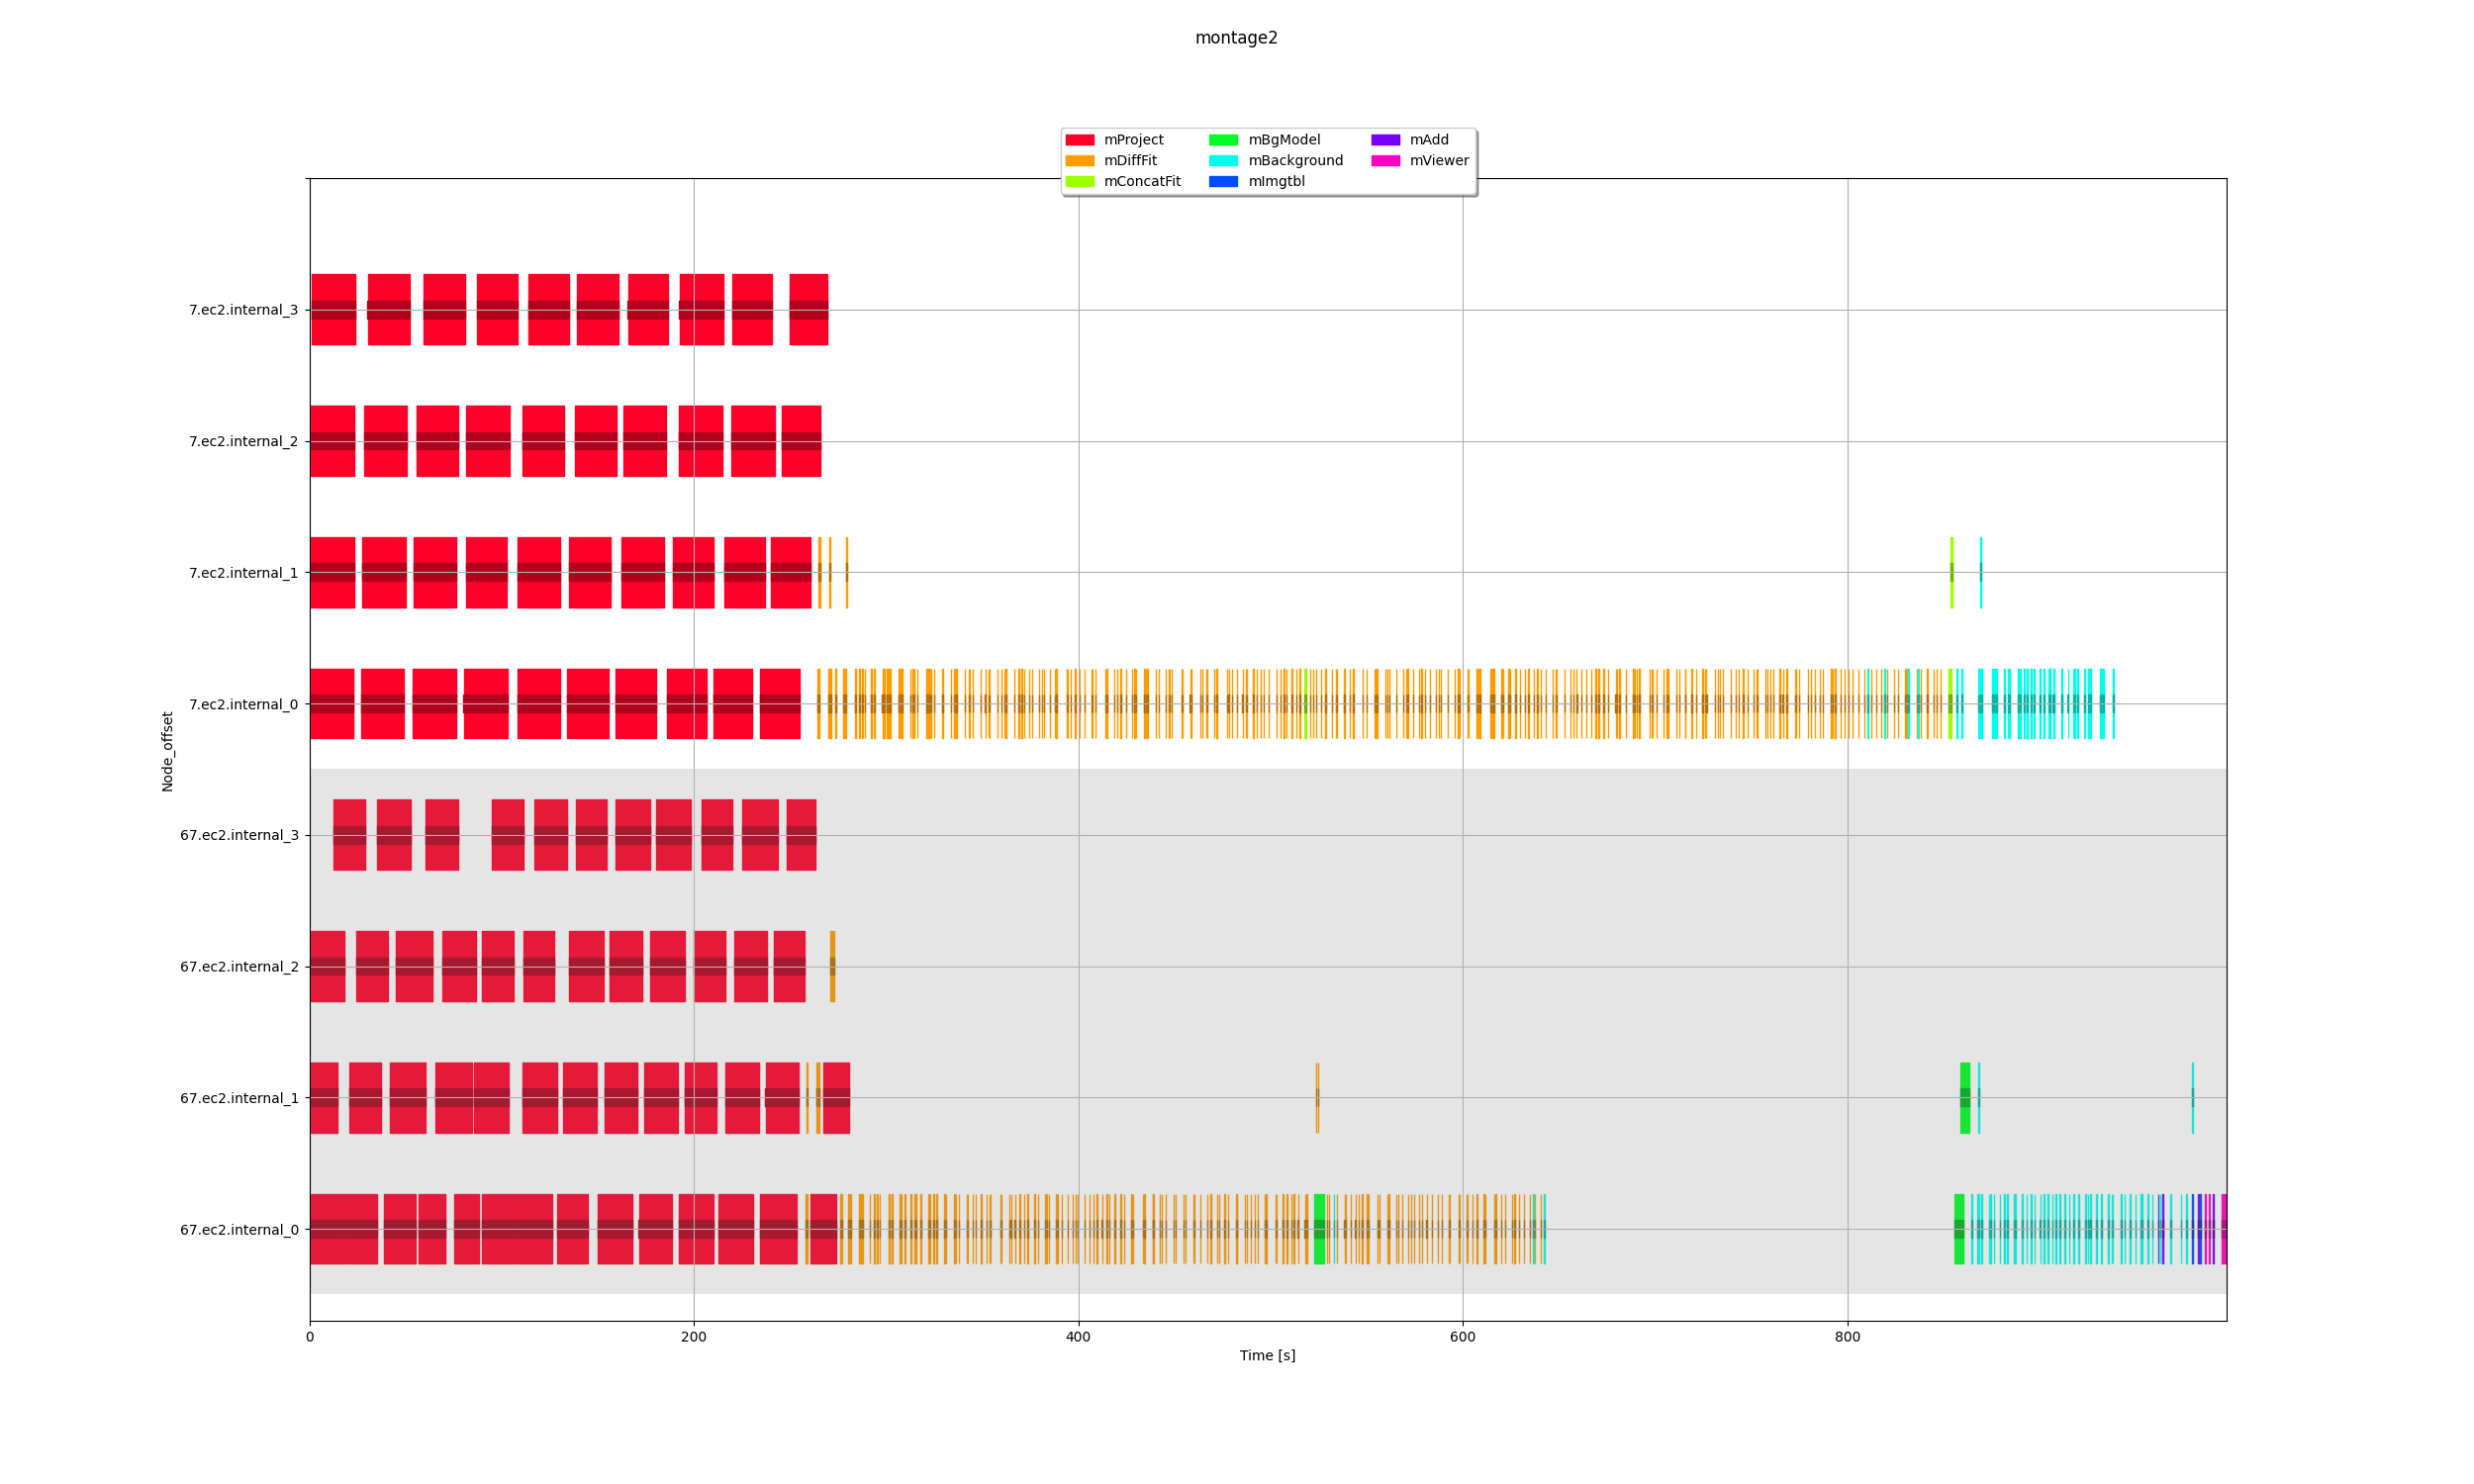
\includegraphics[width=0.75\linewidth]{figures/6-1-m0.25-heft.png}
        \caption[Selected example execution traces for Montage2-v0.25 workflow with HEFT]{HEFT}
        \label{fig:evaluation:sched:m025:heft}
    \end{subfigure}
%%
    \begin{subfigure}{1\textwidth}
        \centering
        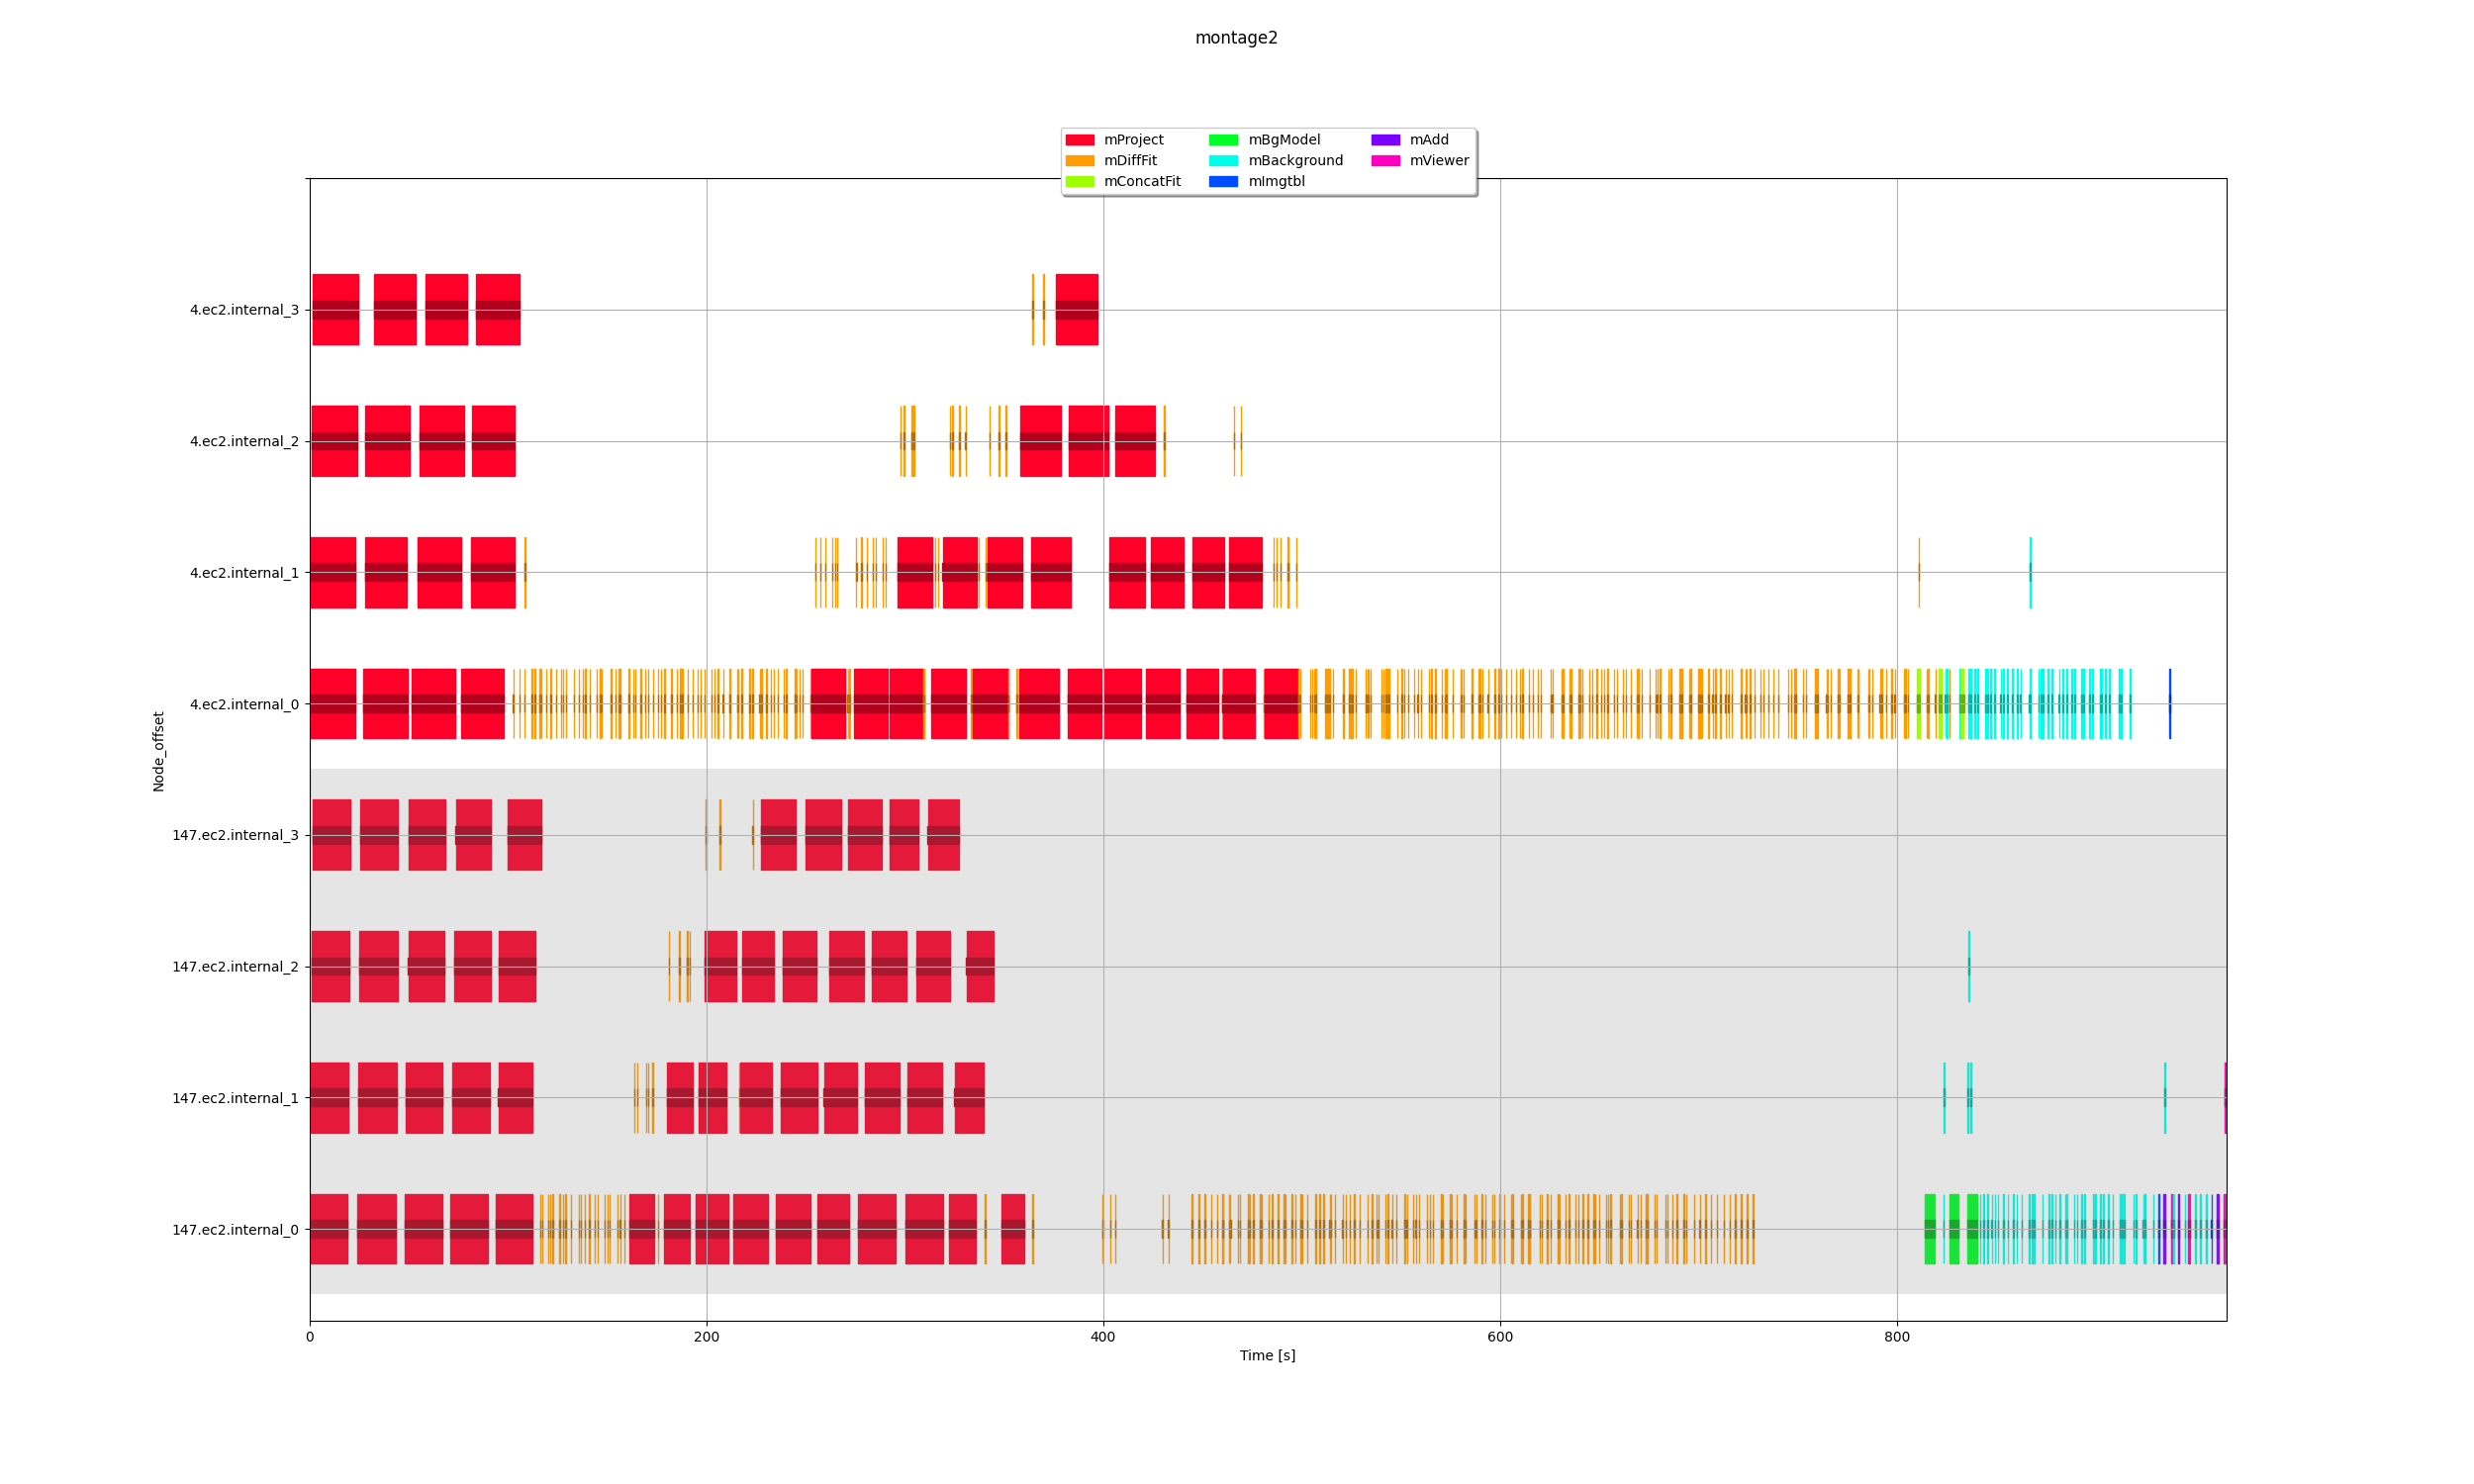
\includegraphics[width=0.75\linewidth]{figures/6-1-m0.25-peft.png}
        \caption[Selected example execution traces for Montage2-v0.25 workflow with PEFT]{PEFT}
        \label{fig:evaluation:sched:m025:peft}
    \end{subfigure}
%%
    \centering
%%
    \caption[Selected example execution traces for Montage2-v0.25 workflow]{Selected example execution traces for Montage2-v0.25.}
%%
    \label{fig:evaluation:sched:m025:plugin}
\end{figure} %%%%%%%
\noindent
Following the trace of the default solution, the longer tasks (\emph{mProject}) are more scattered in time, lessening the load on the Kubernetes components and allowing for a slightly better workload distribution across available computing units.
The same reasoning could also apply to the PEFT execution analysis, however, the \emph{mProject} tasks have still been packed together relatively tight in a schedule, and have not been interjected between \emph{mDiffFit} tasks to such an extent as in the default solution.
Regarding HEFT schedules for Montage workflow, they seem to prioritize finishing tasks based on the length of the path to the root job.
This way, all \emph{mProject} tasks have been assigned the highest priority and finished before \emph{mDiffFit} ones, which have ended with the lowest possible effective task parallelization.

